\documentclass[a4paper,12pt]{article}
\usepackage{HomeWorkTemplate}
\usepackage{circuitikz}
\usepackage[shortlabels]{enumitem}
\usepackage{hyperref}
\usepackage{tikz}
\usepackage{amsmath}
\usepackage{amssymb}
\usepackage{tcolorbox}
\usepackage{xepersian}
\settextfont{XB Niloofar}
\usetikzlibrary{arrows,automata}
\usetikzlibrary{circuits.logic.US}
\usepackage{changepage}
\newcounter{problemcounter}
\newcounter{subproblemcounter}
\setcounter{problemcounter}{1}
\setcounter{subproblemcounter}{1}
\newcommand{\problem}[1]
{
	\subsection*{
		پرسش
		\arabic{problemcounter} 
		\stepcounter{problemcounter}
		\setcounter{subproblemcounter}{1}
		#1
	}
}
\newcommand{\subproblem}{
	\textbf{\harfi{subproblemcounter})}\stepcounter{subproblemcounter}
}

\usepackage{adjustbox}

\begin{document}
\handout
{شبکه‌های کامپیوتری}
{دکتر لاله ارشدی}
{نیم‌سال اول 1399\lr{-}1400}
{اطلاعیه}
{آئیریا محمدی}
{۹۷۱۰۳۷۷۹}
 {تمرین سری دوم}

\pararaph {1}

 

\section{TCP}
\problem{}
\begin{figure}	
\end{figure}

\begin{align*}
	&\text{IP: } 192.168.1.102 \\
	&\text{Port: } 1161
\end{align*}

{
\centering
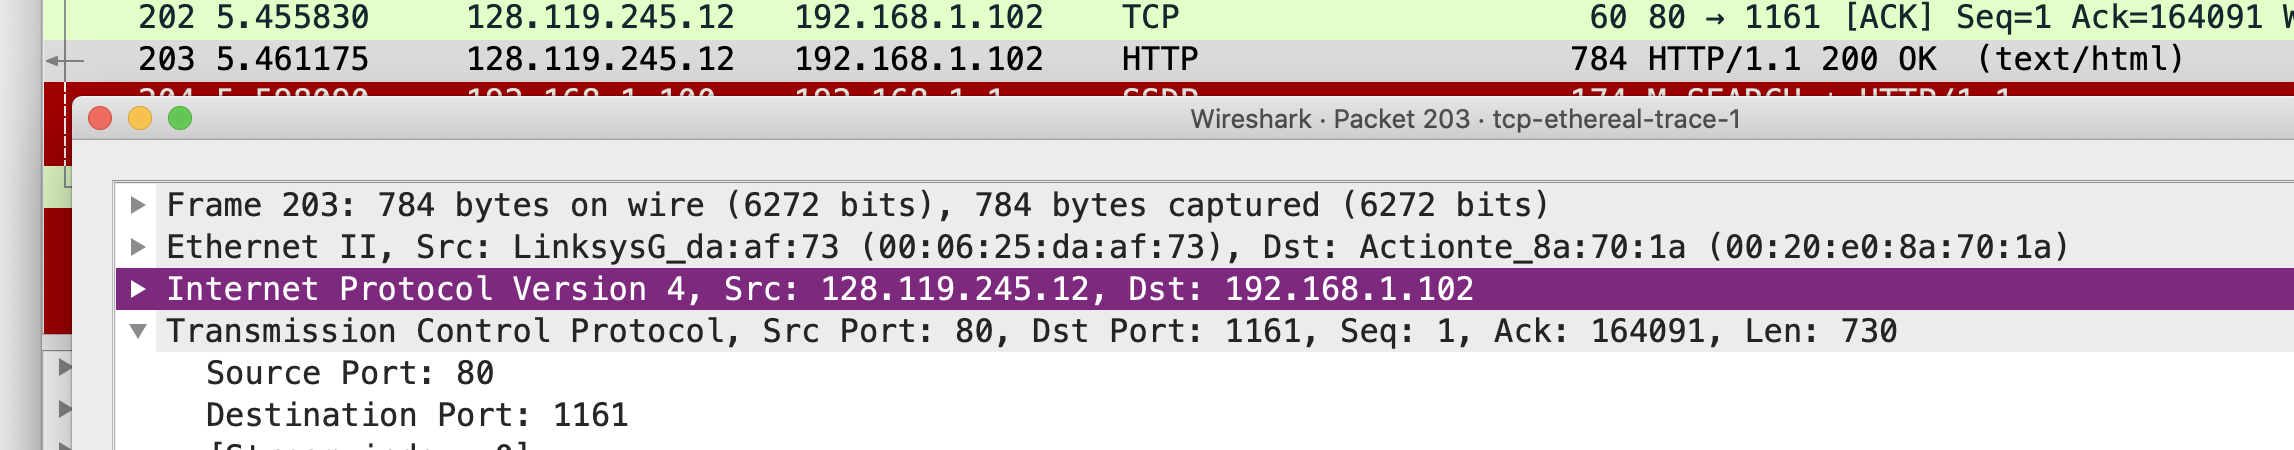
\includegraphics[scale = 0.4]{s1}
}

\problem{}

\begin{align*}
	&\text{IP: } 128.119.245.12 \\
	&\text{Port: } 80
\end{align*}

{
\centering
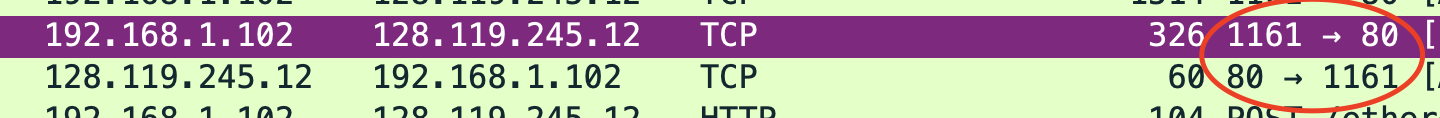
\includegraphics[scale = 0.6]{s2}
}

\problem{}

{
\centering
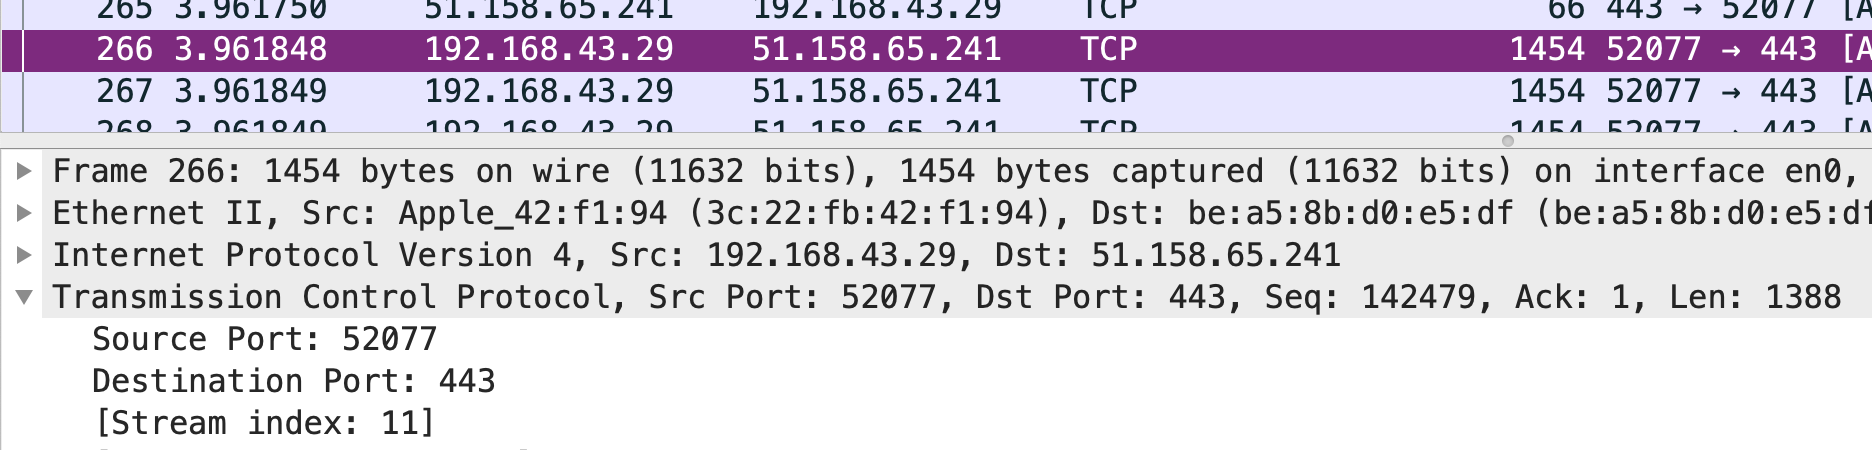
\includegraphics[scale = 0.50]{s3}
}

\begin{align*}
	&\text{IP: } 192.168.43.29 \\
	&\text{Port: } 52077
\end{align*}

\problem{}

{
\centering
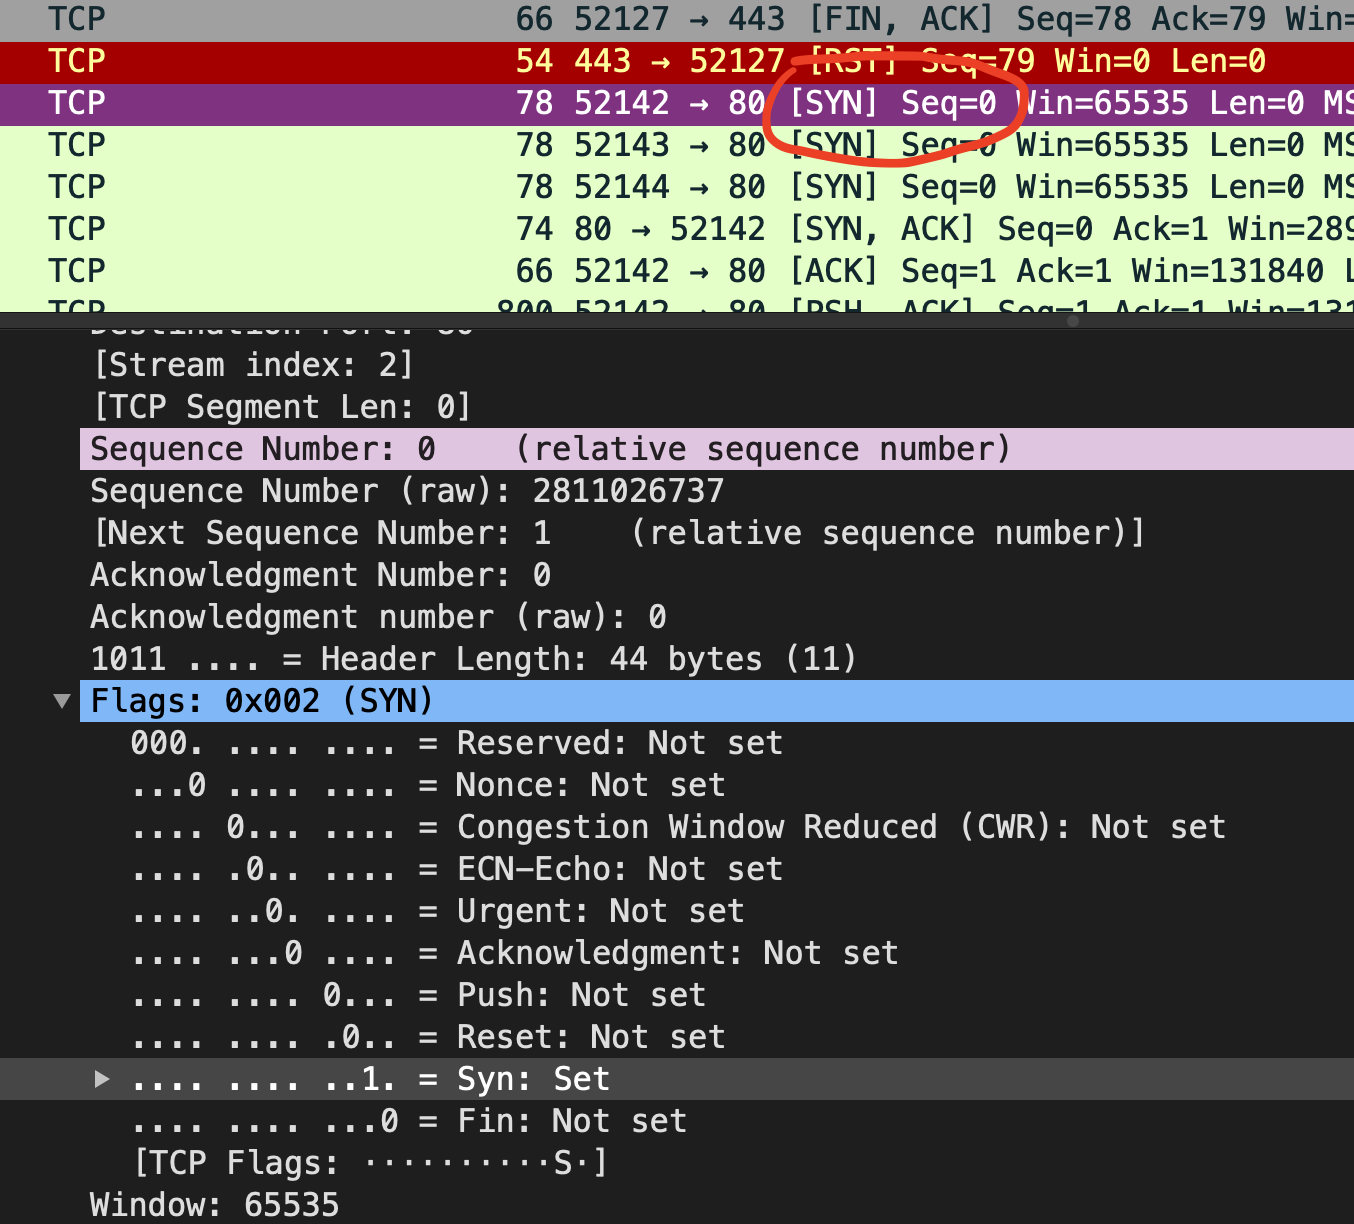
\includegraphics[scale = 0.65]{s4} \\
\begin{latin}
a) sequence number = 0 \\
b) the sequence number being zero and the syn flag being set.
\end{latin}
}

\problem{}
{
\centering
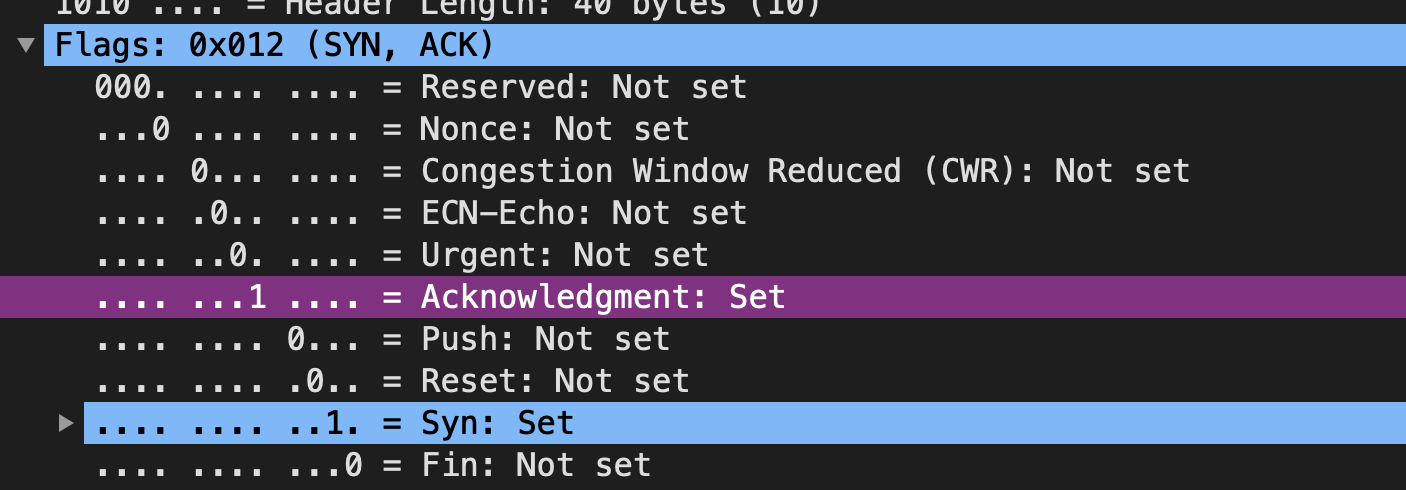
\includegraphics[scale = 0.65]{s5} \\
\begin{latin}
(check previous figure) the sequence number is 0 in response to syn segment). \\
the value of acknowledgement field in synack is 1 (1+ sender sequence number). \\
the syn and ack fields being set to 1.
\end{latin}
}

\problem{}

{
\centering
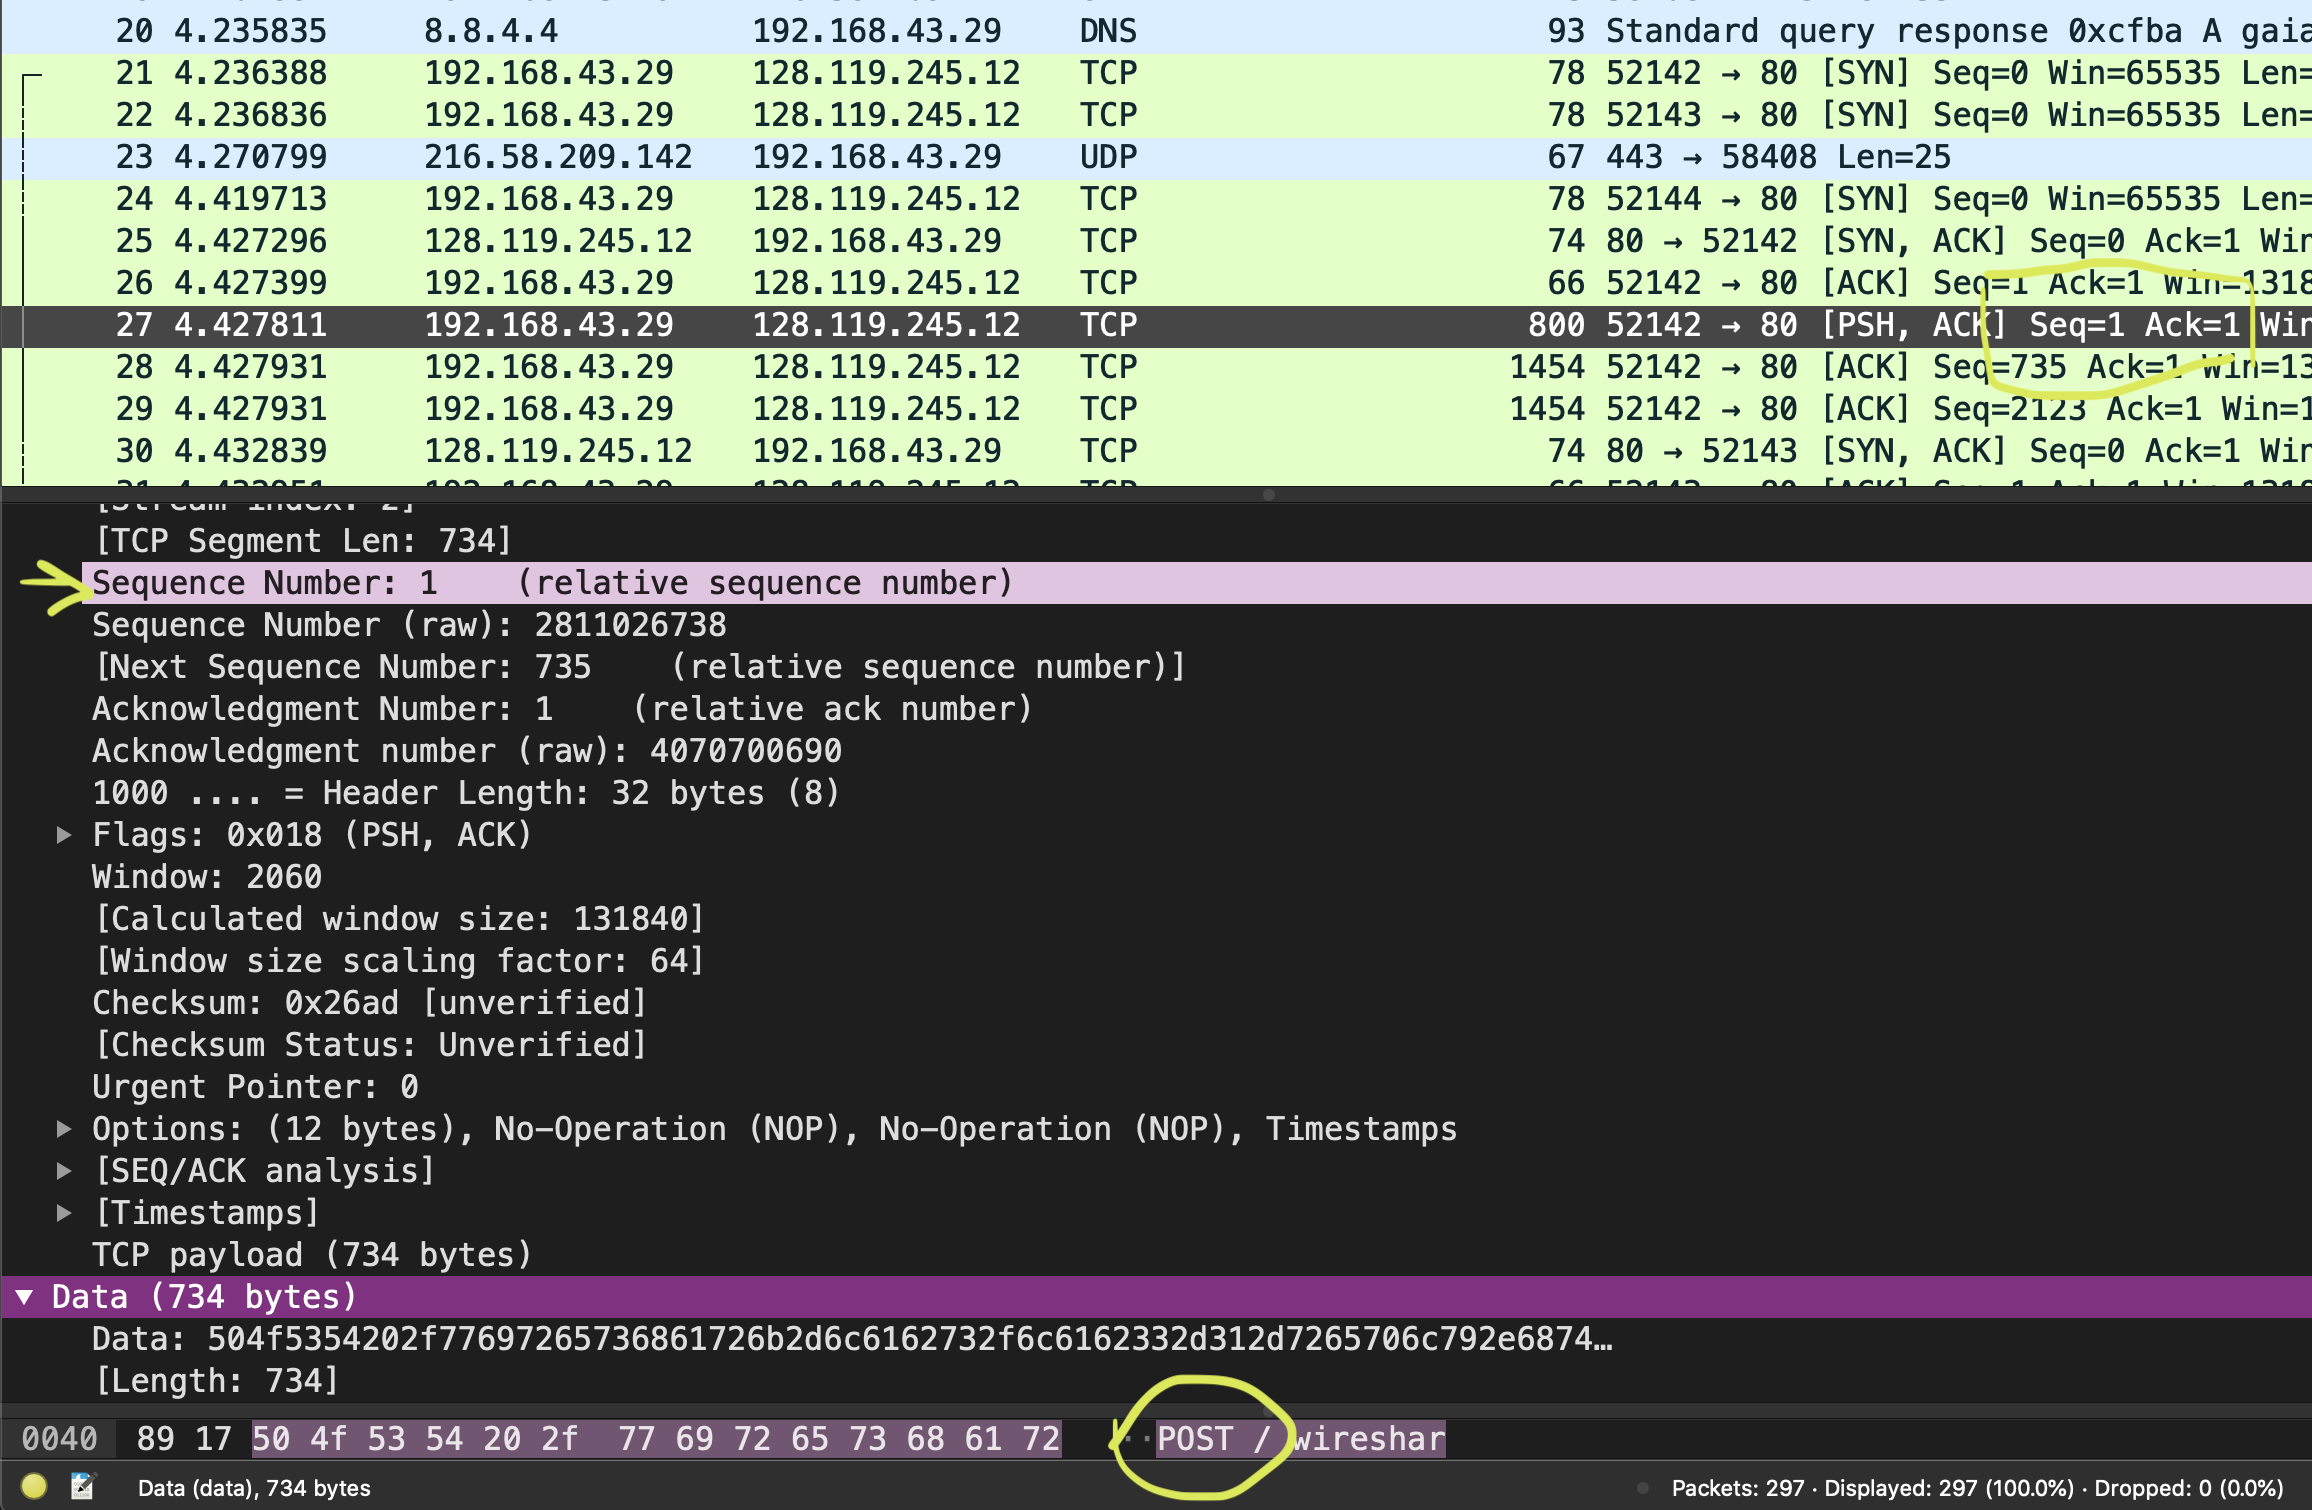
\includegraphics[scale = 0.39]{s6.png}} \\
\begin{latin}
sequence number = 1	
\end{latin}
}

\problem{}

\begin{latin}
\begin{tabular}{ |p{2cm}|p{2cm}|p{2cm}|p{2cm}|p{3cm}|  }
 \hline
Seq \# & Send &Receive
 &
 RTT & Estimated RTT \\
 \hline
 1 & 4.427811 & 4.626372 & 0.198561 & 0.198561 \\ 
 735 & 4.427931 & 4.629205 & 0.201274 & 0.198900 \\
 2123 & 4.427931 & 4.631127 & 0.203196 & 0.199437 \\
 3511 & 4.626465 & 4.933905 & 0.307440 & 0.212937 \\
 4899 & 4.629273 & 4.933909 & 0.304636 & 0.224399 \\
 6287 & 4.629273 & 4.933910 & 0.304636 & 0.234429 \\
 \hline
\end{tabular}
\end{latin}

\begin{figure}
	\centering
	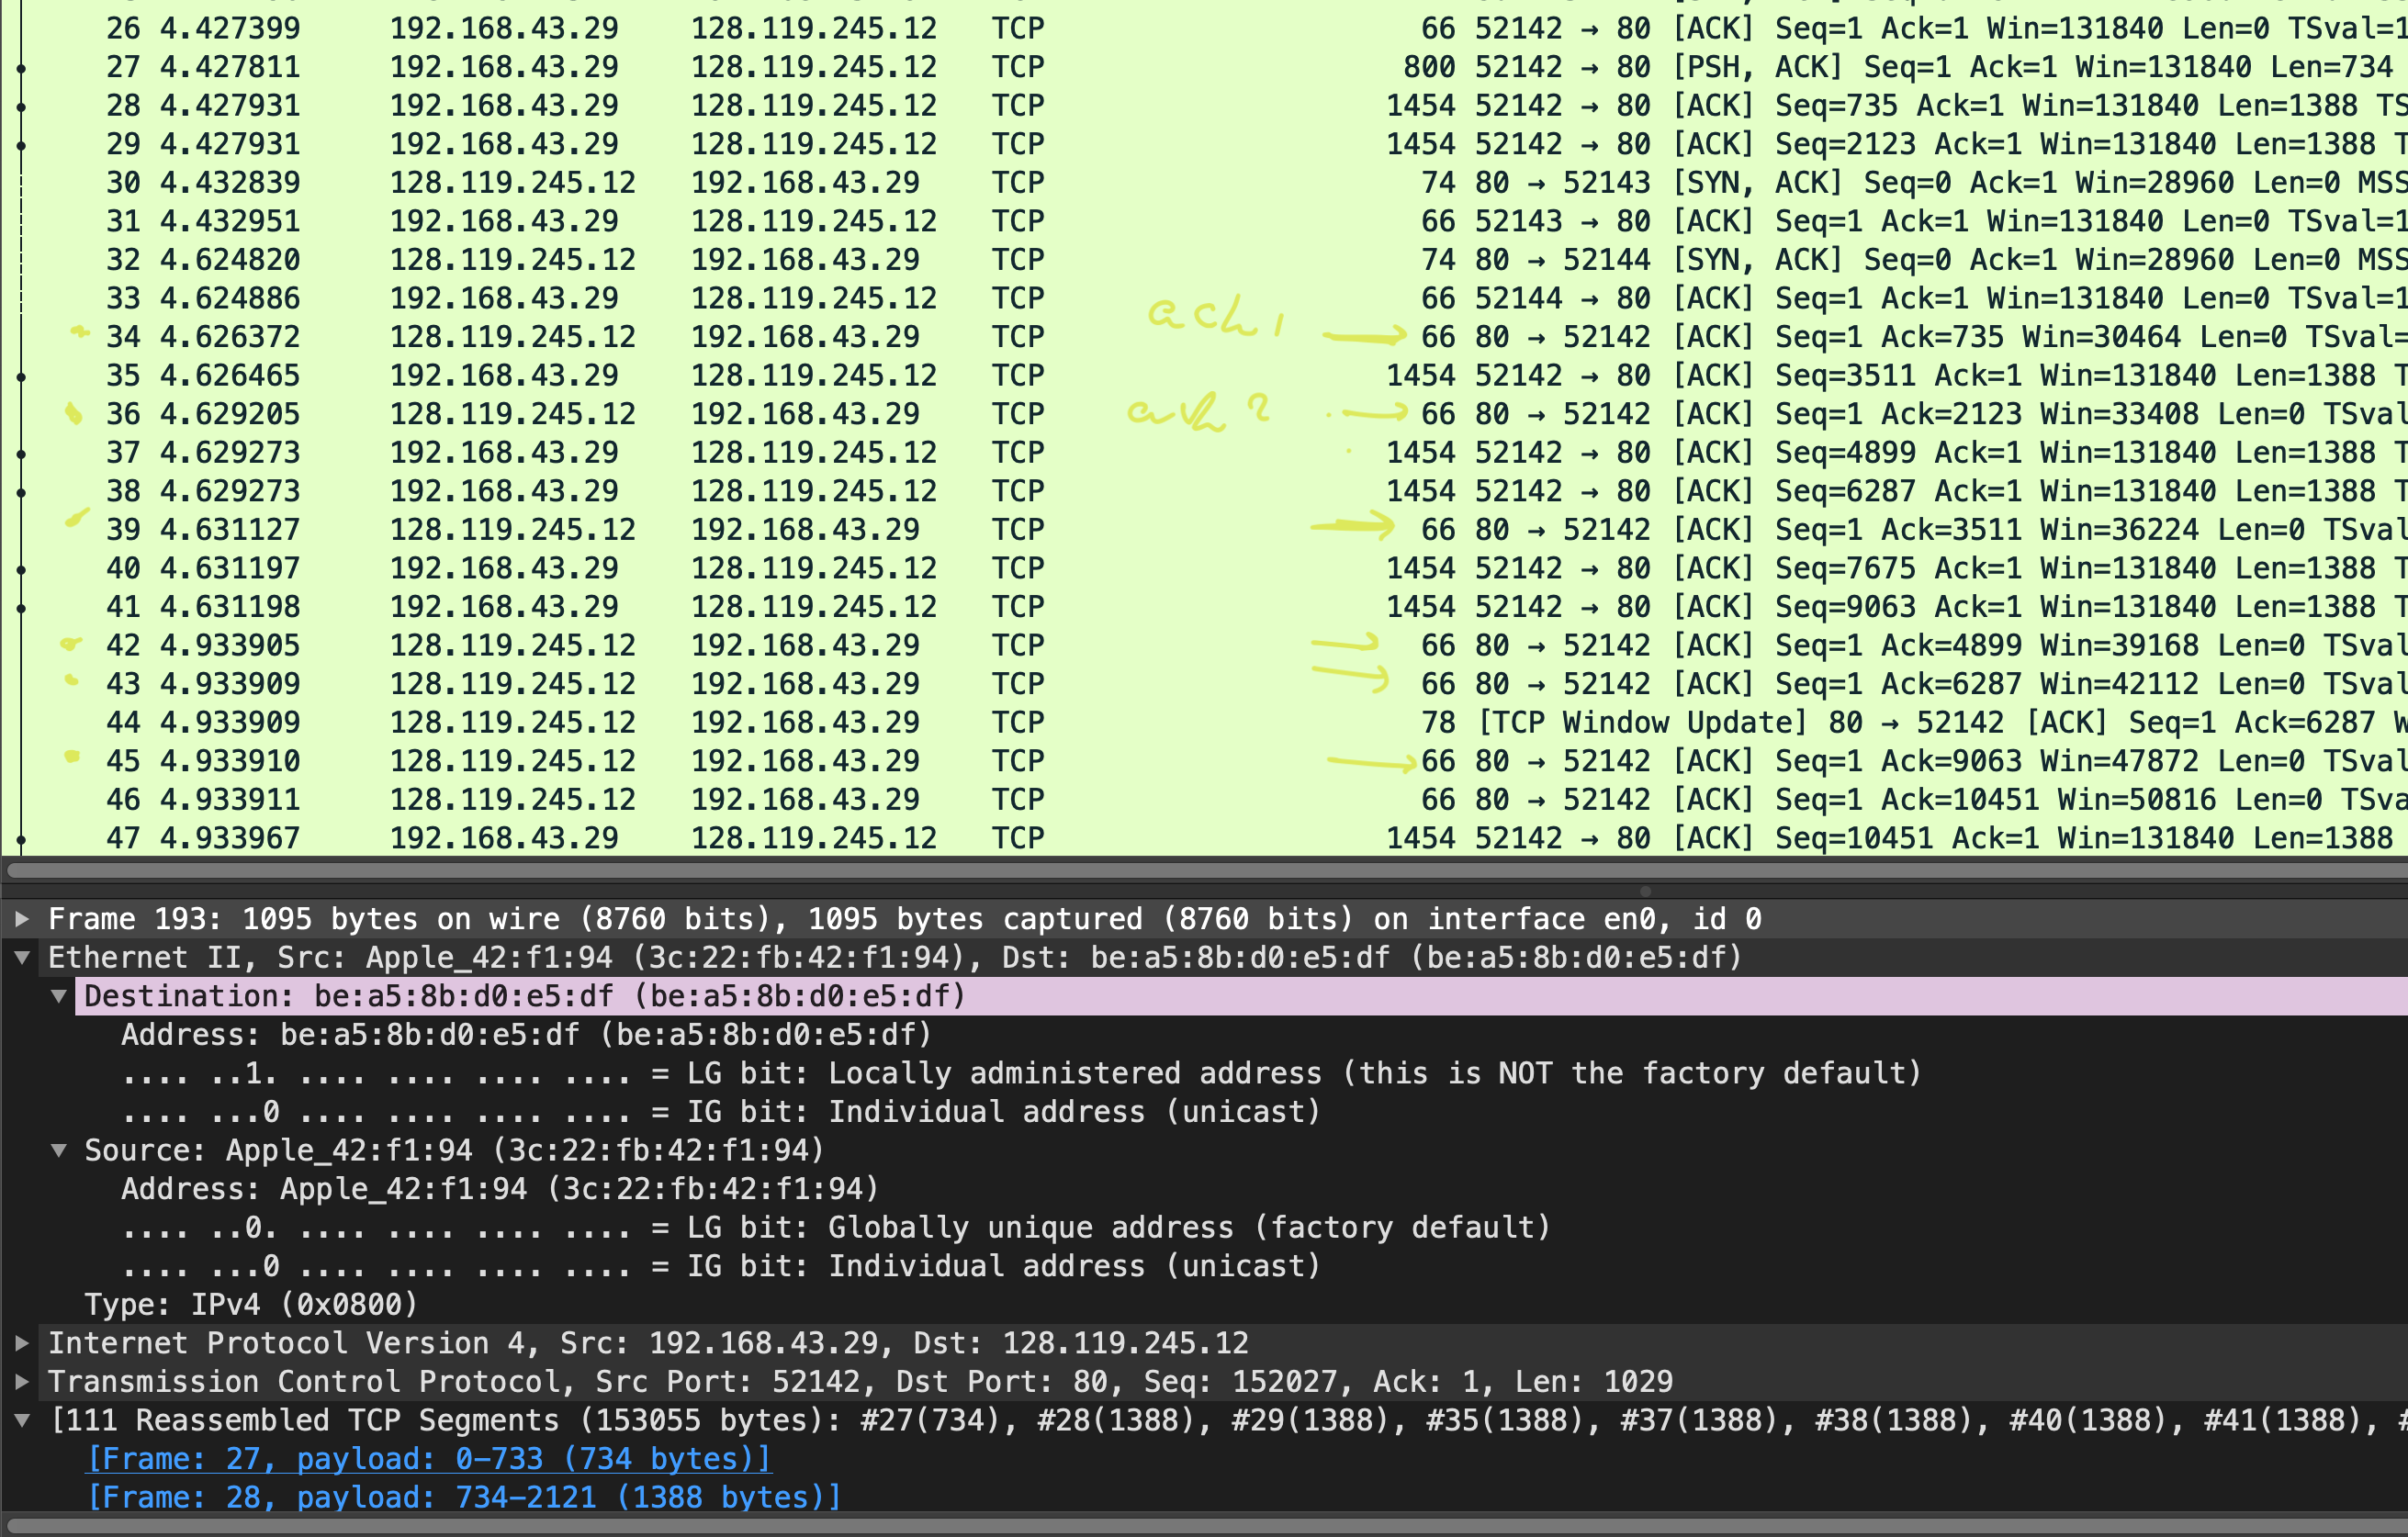
\includegraphics[scale= 0.35]{s7}
	\caption{\lr{packets of http message shown with dot} }
\end{figure}

\begin{figure}
\centering
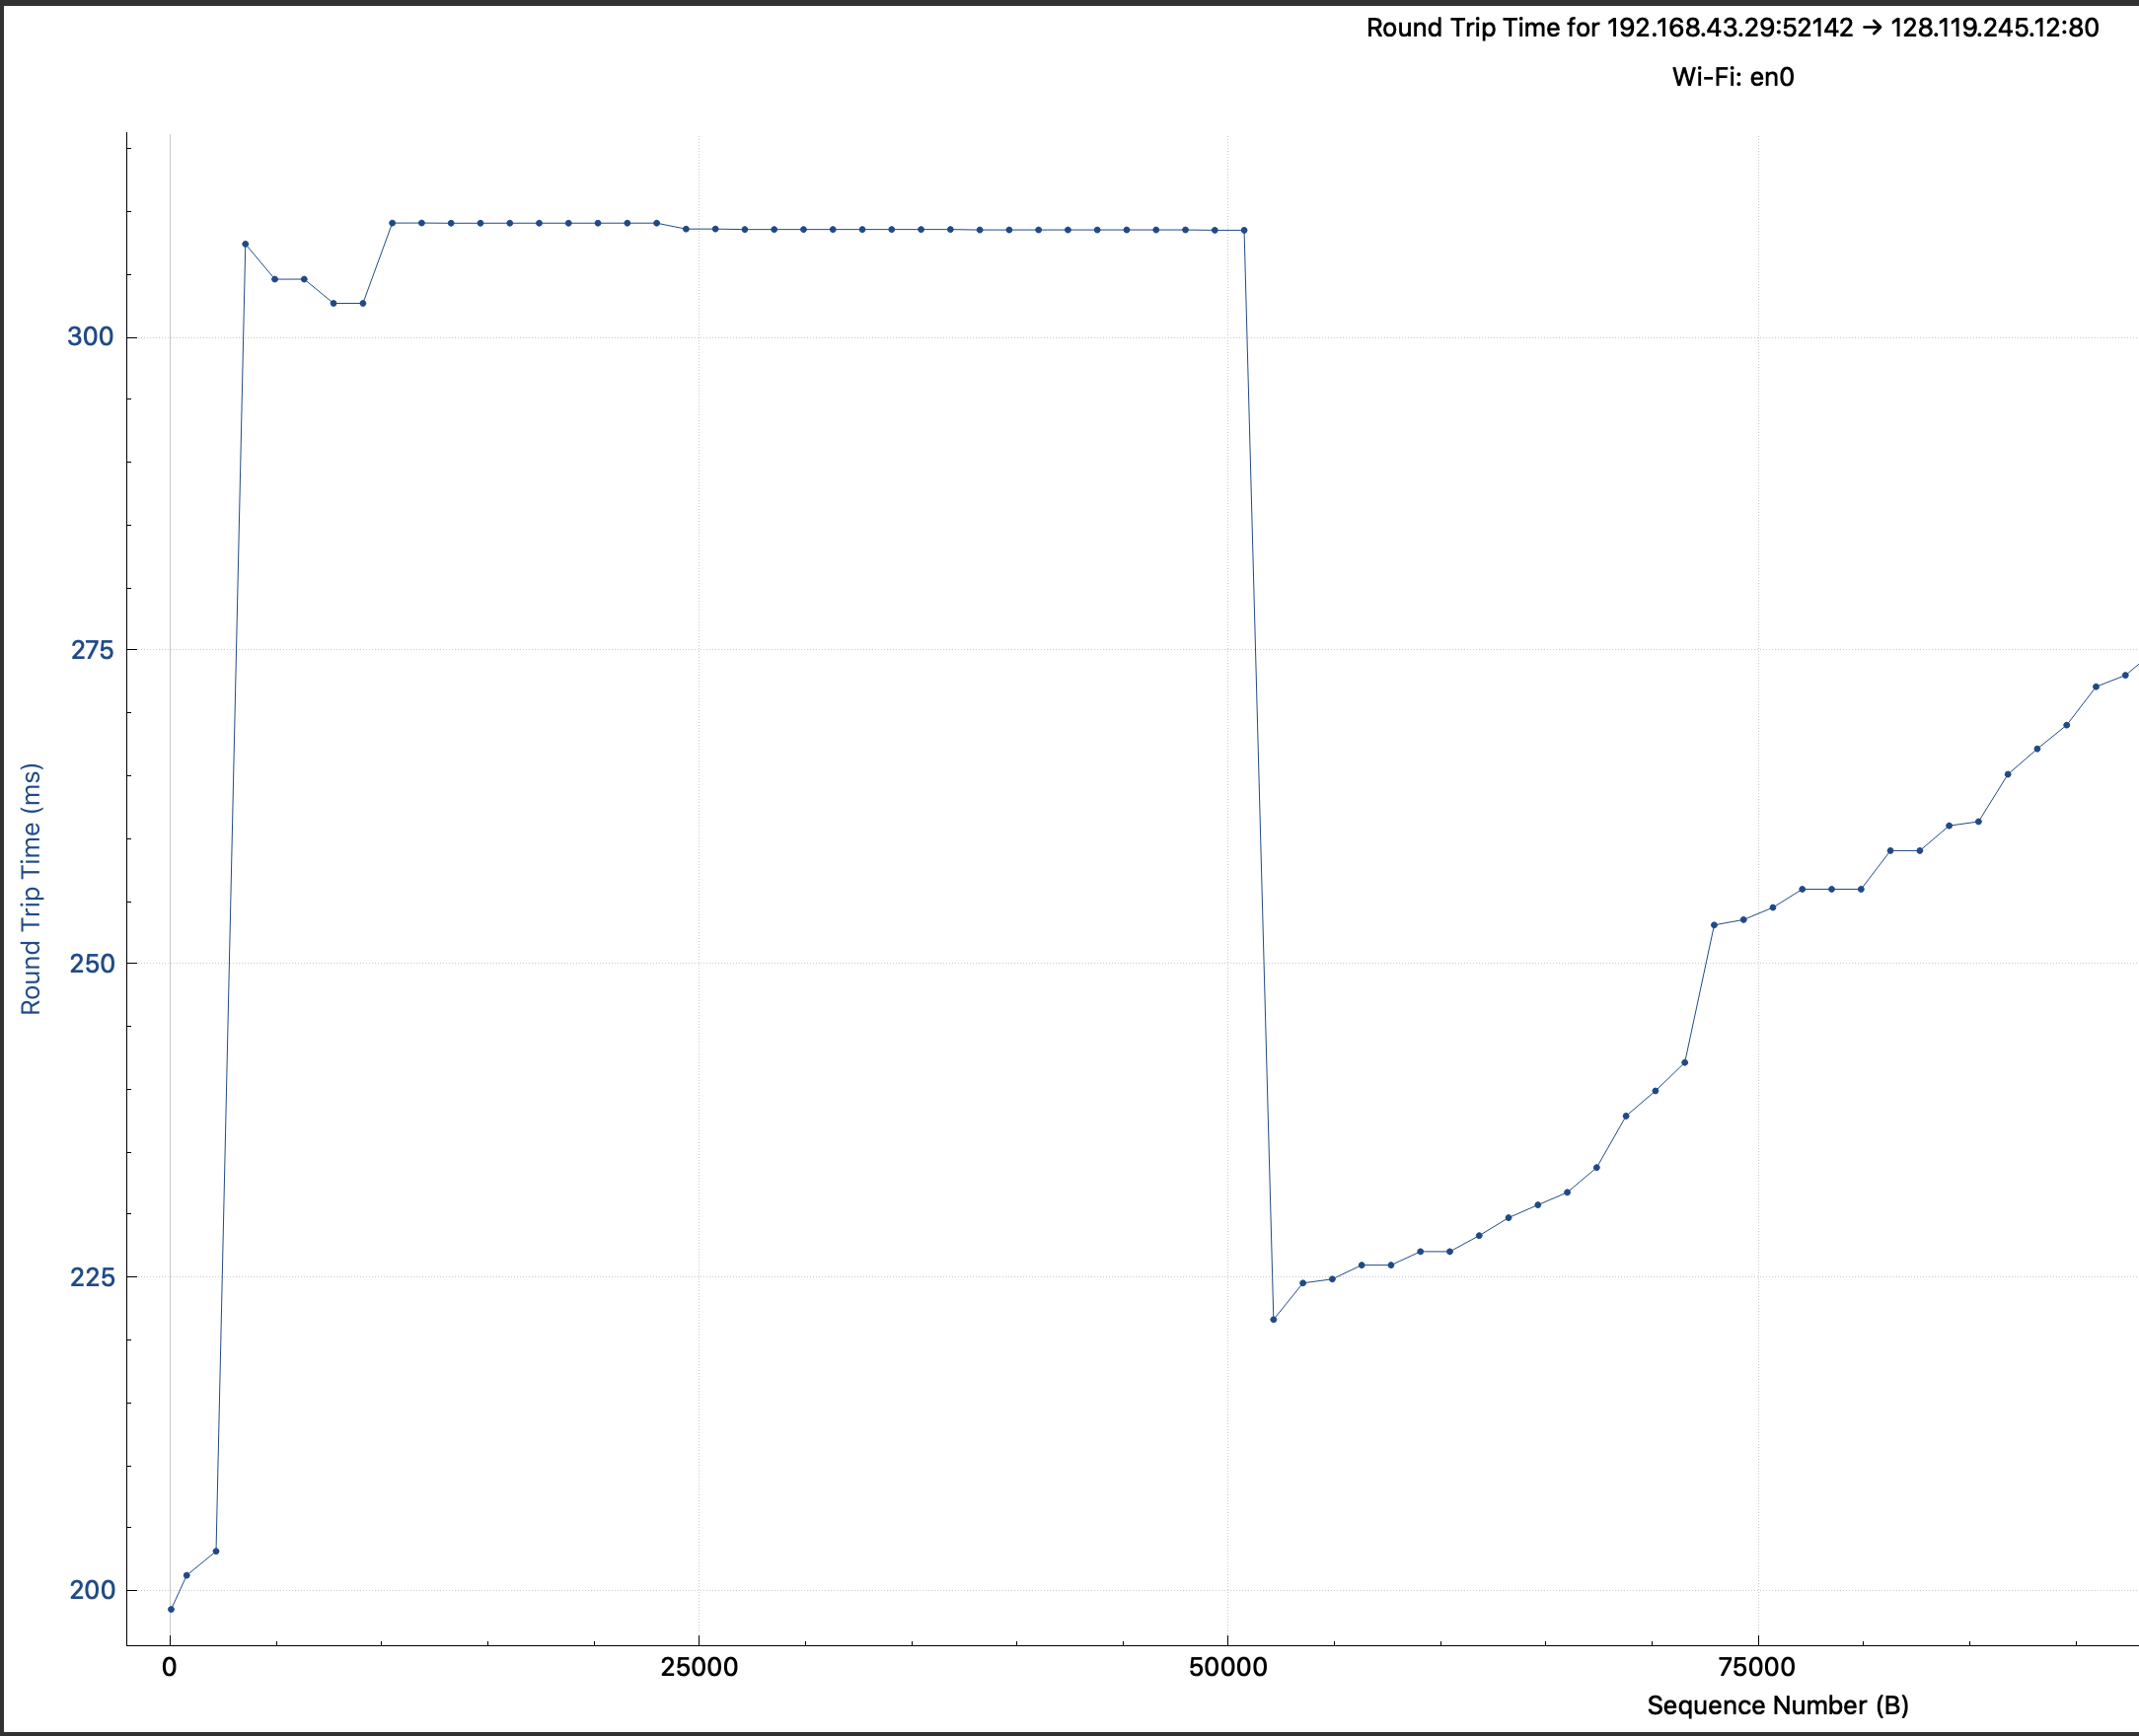
\includegraphics[scale=0.32]{tcp-graph}
\caption{\lr{RTT Change}}
\end{figure}

\problem{}
 
 
\begin{figure}
	\centering
	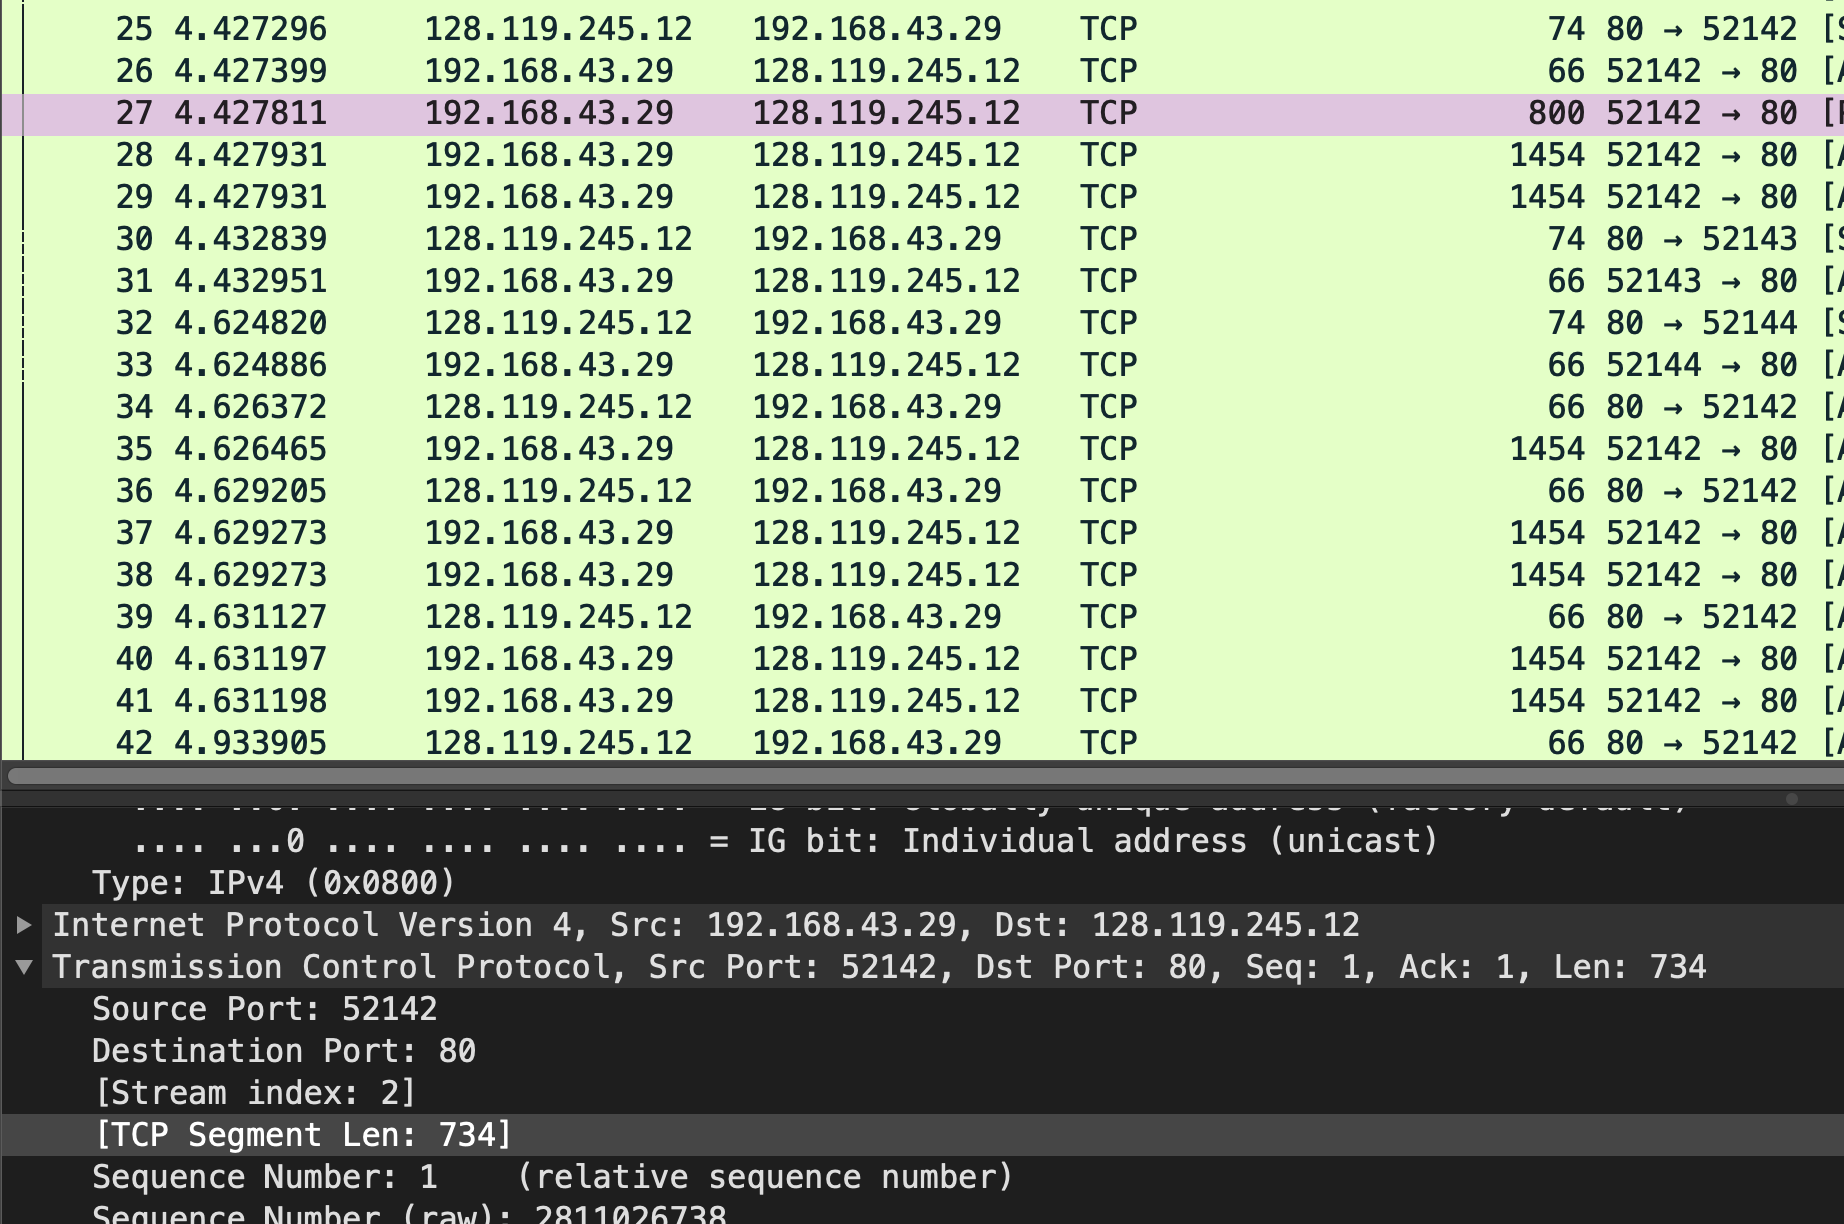
\includegraphics[scale= 0.53]{s8-1.png}
	\caption{\lr{tcp segment len: 734} }
\end{figure}

\begin{figure}
	\centering
	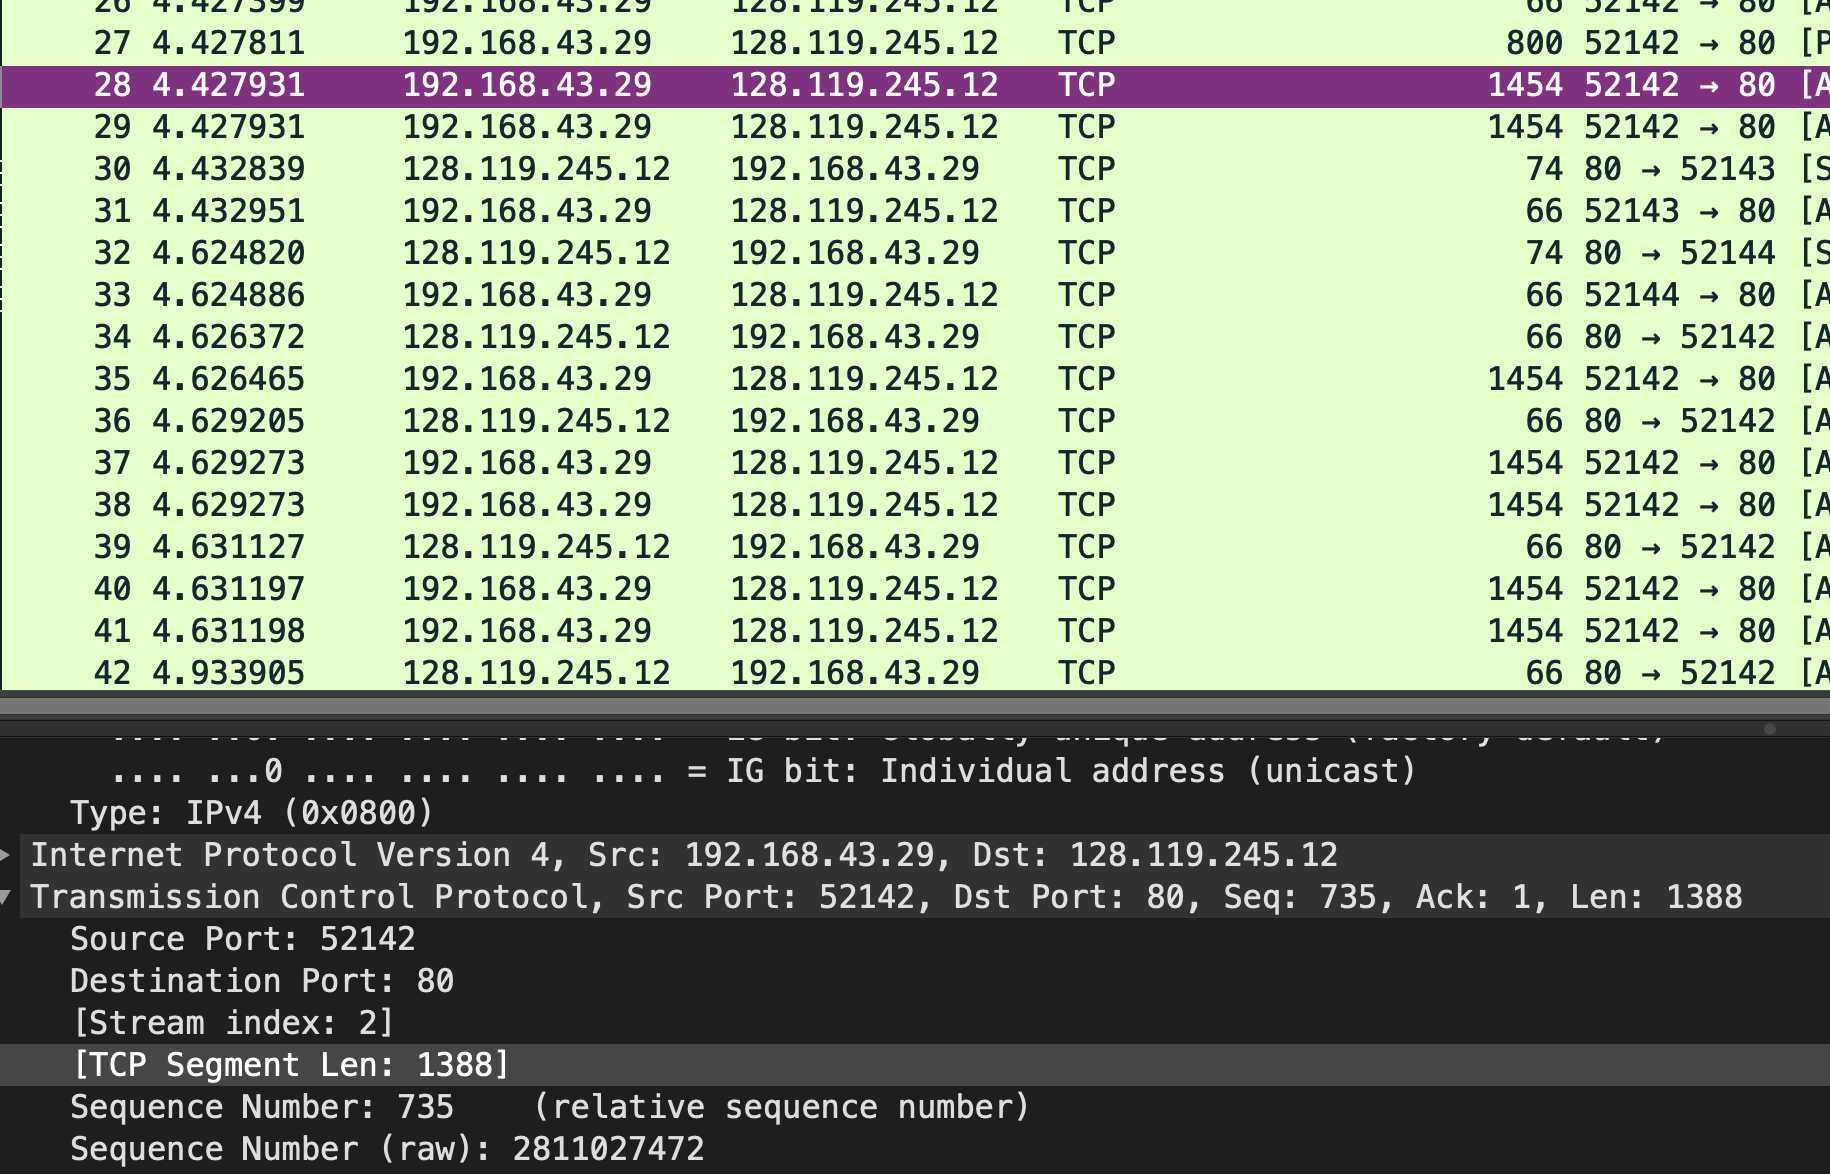
\includegraphics[scale= 0.53]{s8-2.png}
	\caption{\lr{tcp segment len of the rest: 1388} }
\end{figure}

\begin{figure}
	\centering
	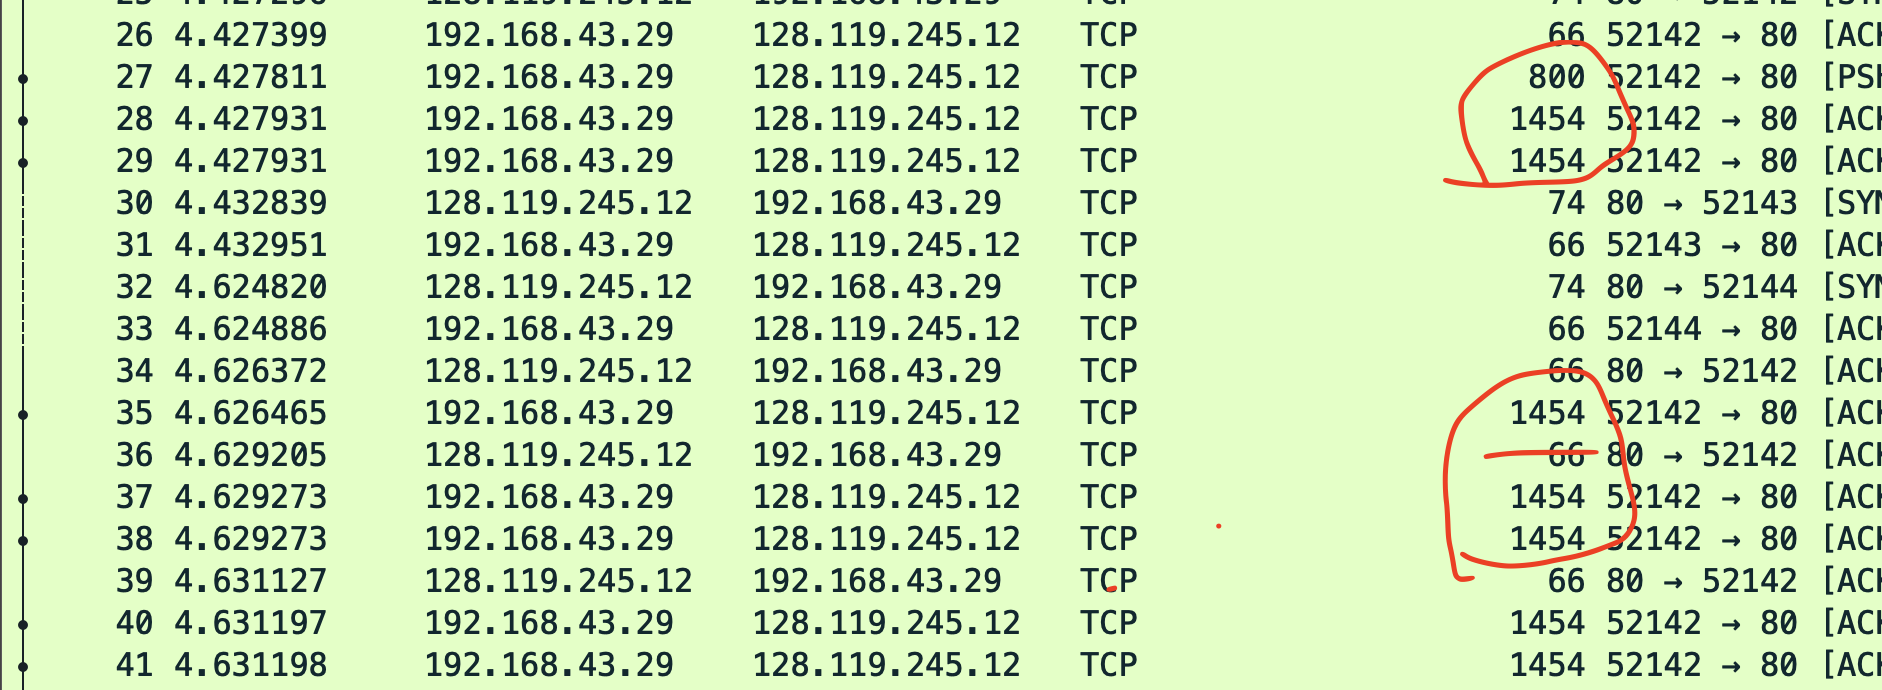
\includegraphics[scale= 0.53]{s8.png}
	\caption{\lr{len with headers: 800, 1454, 1454, 1454, 1454, 1454} }
\end{figure}

\begin{figure}
	\centering
	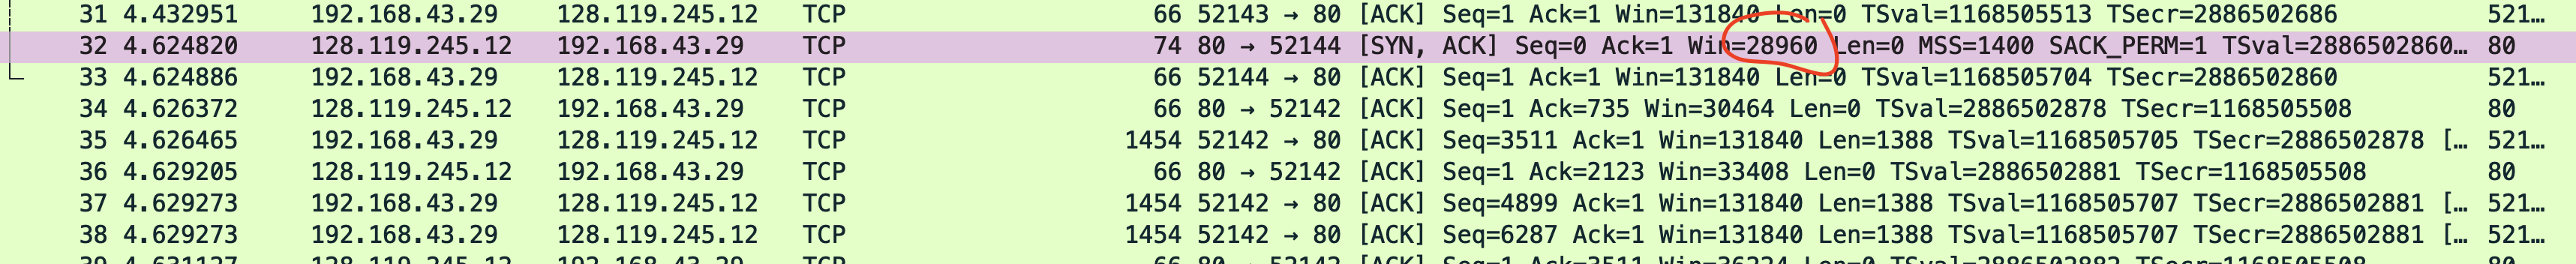
\includegraphics[scale= 0.30]{s9.png}
	\caption{\lr{initial receiver window size of 28960 bytes.\\ sender never throttles because receiver's window size is (far) smaller.}}
\end{figure}


\problem{}

\begin{figure}
	\centering
	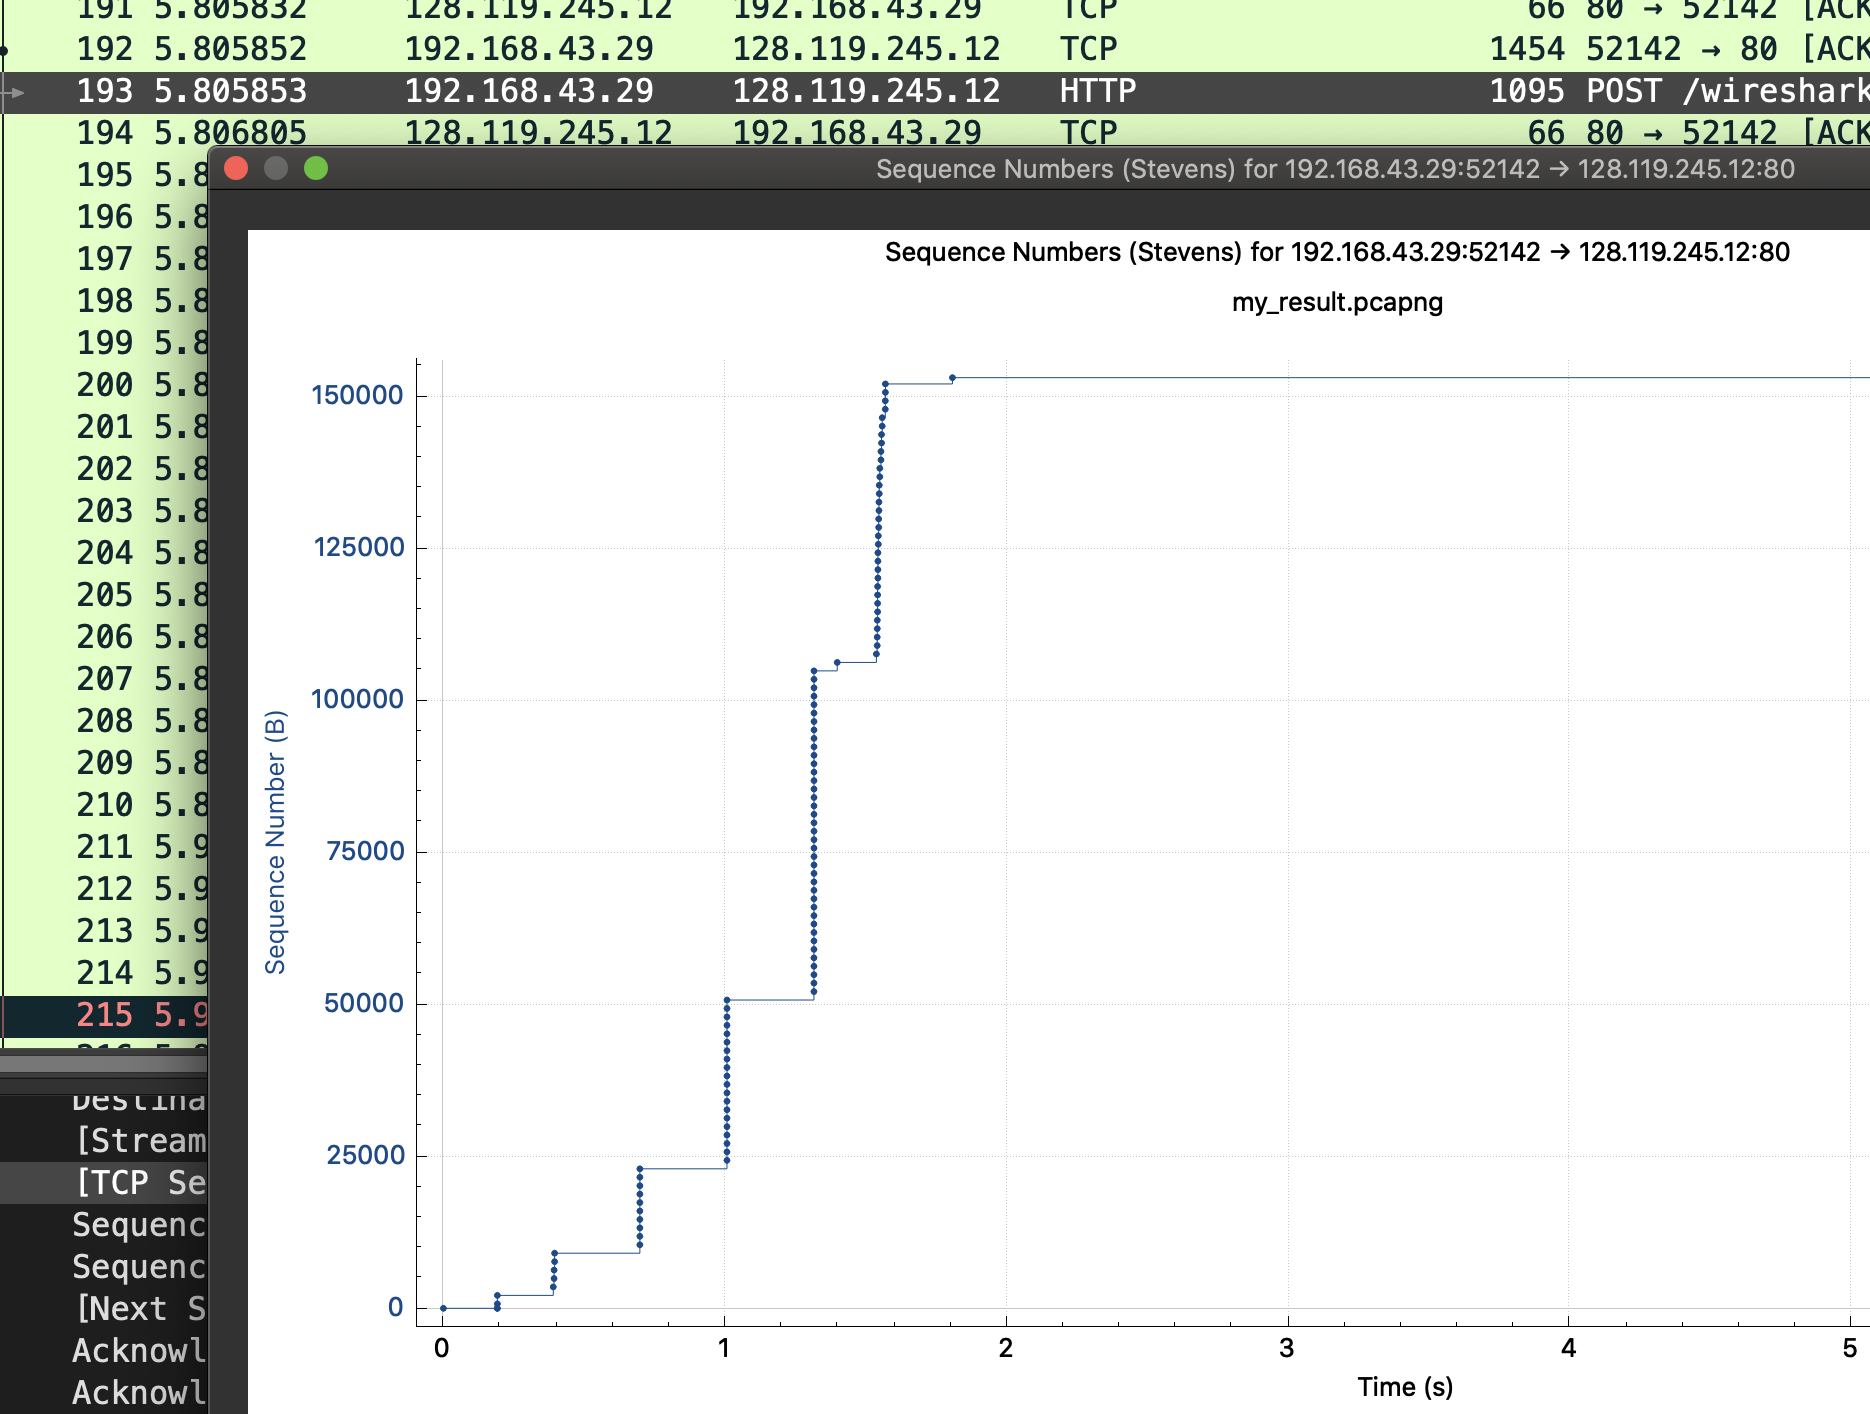
\includegraphics[scale= 0.30]{s10.png}
	\caption{\lr{no, the sequence numbers are only increasing.}}
\end{figure}

\problem{}

\begin{figure}
	\centering
	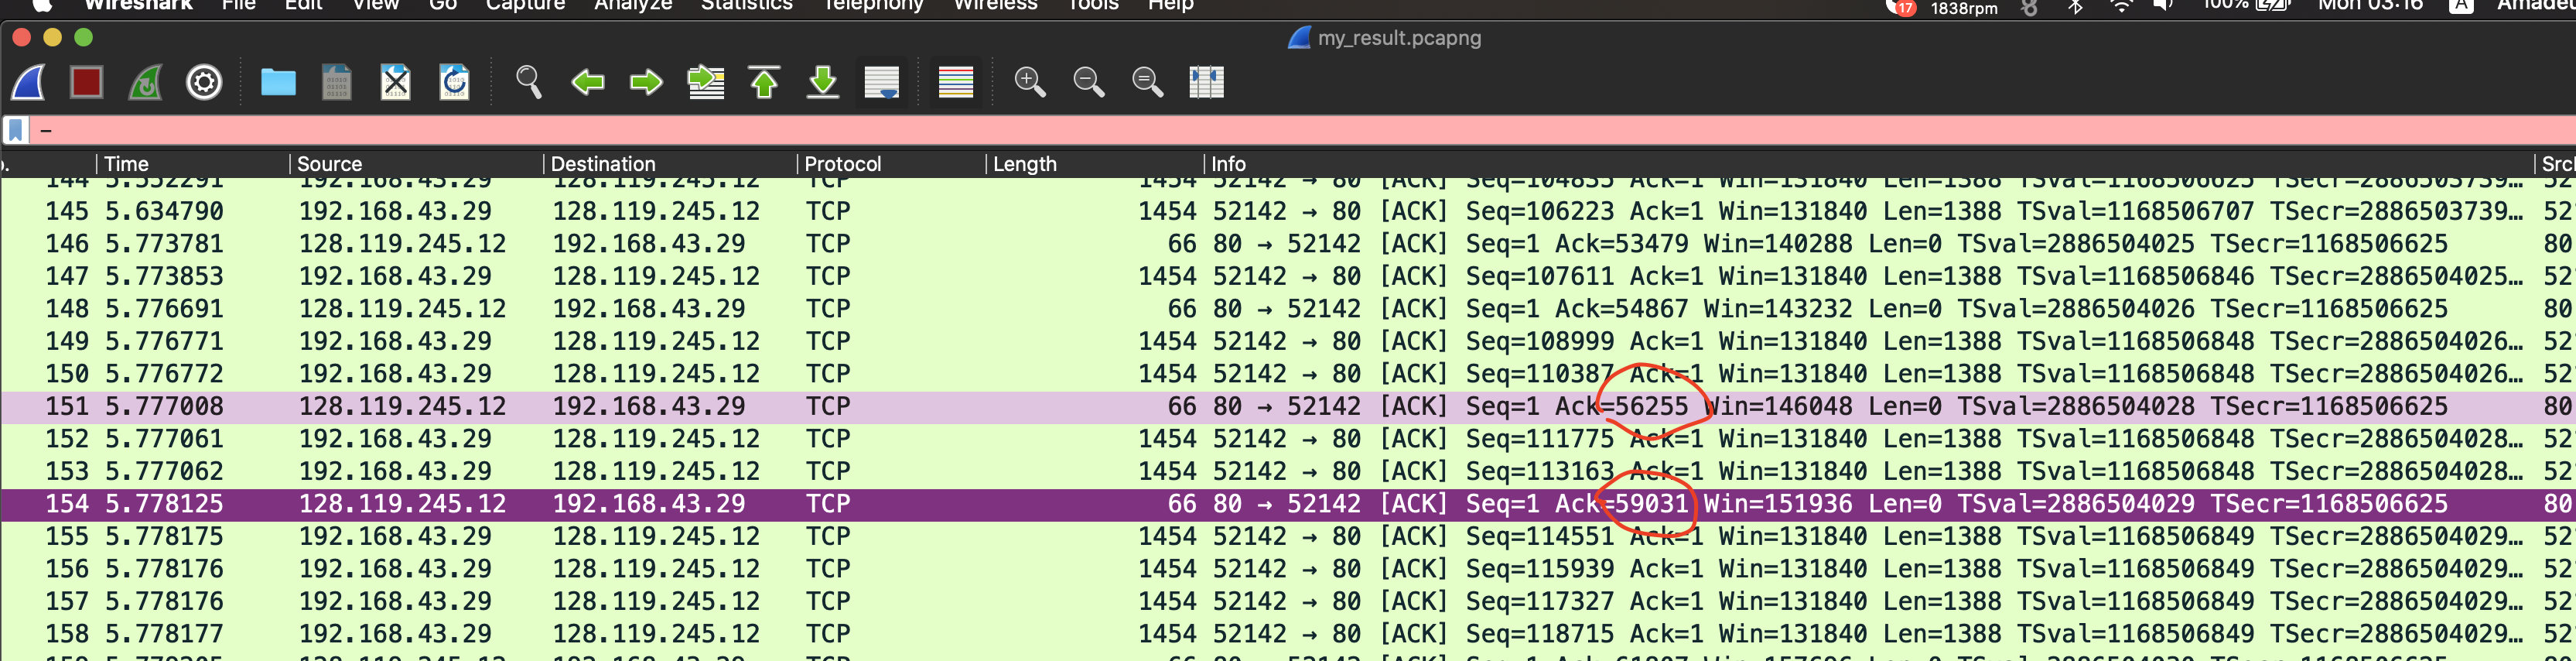
\includegraphics[scale= 0.40]{s11.png}
	\caption{\lr{typically it's 1388 bytes. sometimes (as highlightet) it's more. as it can be seen here more than a packet (two) was acked altogether here.}}
\end{figure}

\problem{}

\begin{figure}
	\centering
	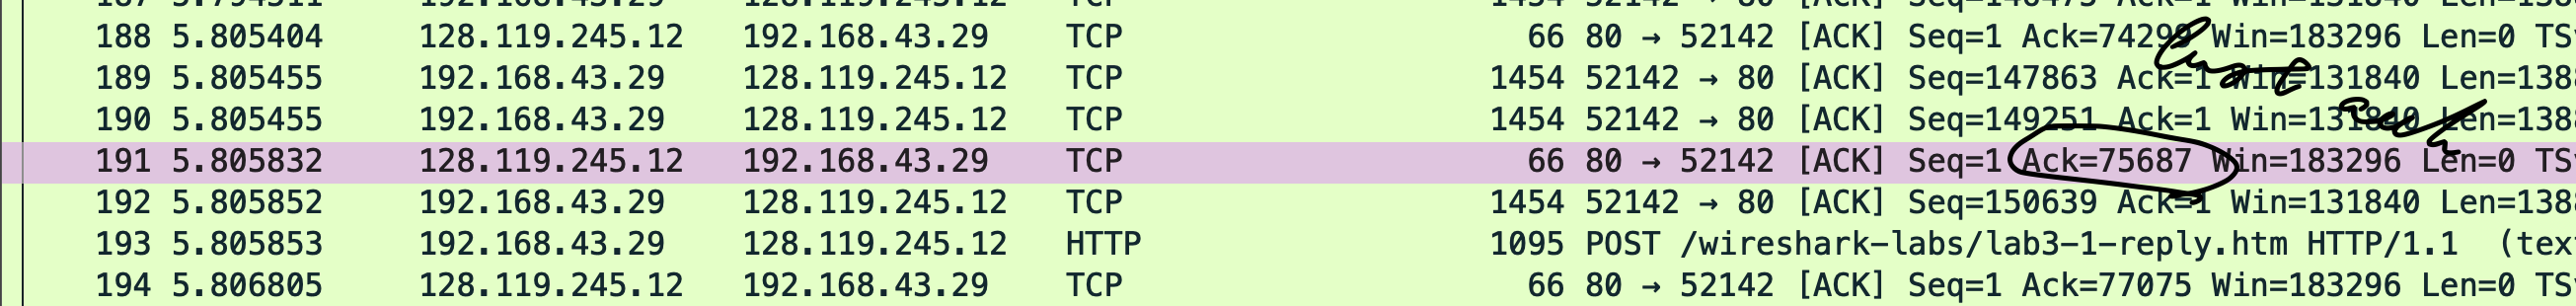
\includegraphics[scale= 0.40]{s12.png}
	\caption{\lr$75687 / (5.8058 - 4.624886) = 64.091 Kbyte/sec$.}}
\end{figure}

\newpage

\section{UDP}

1-\\\\
{
	\centering
	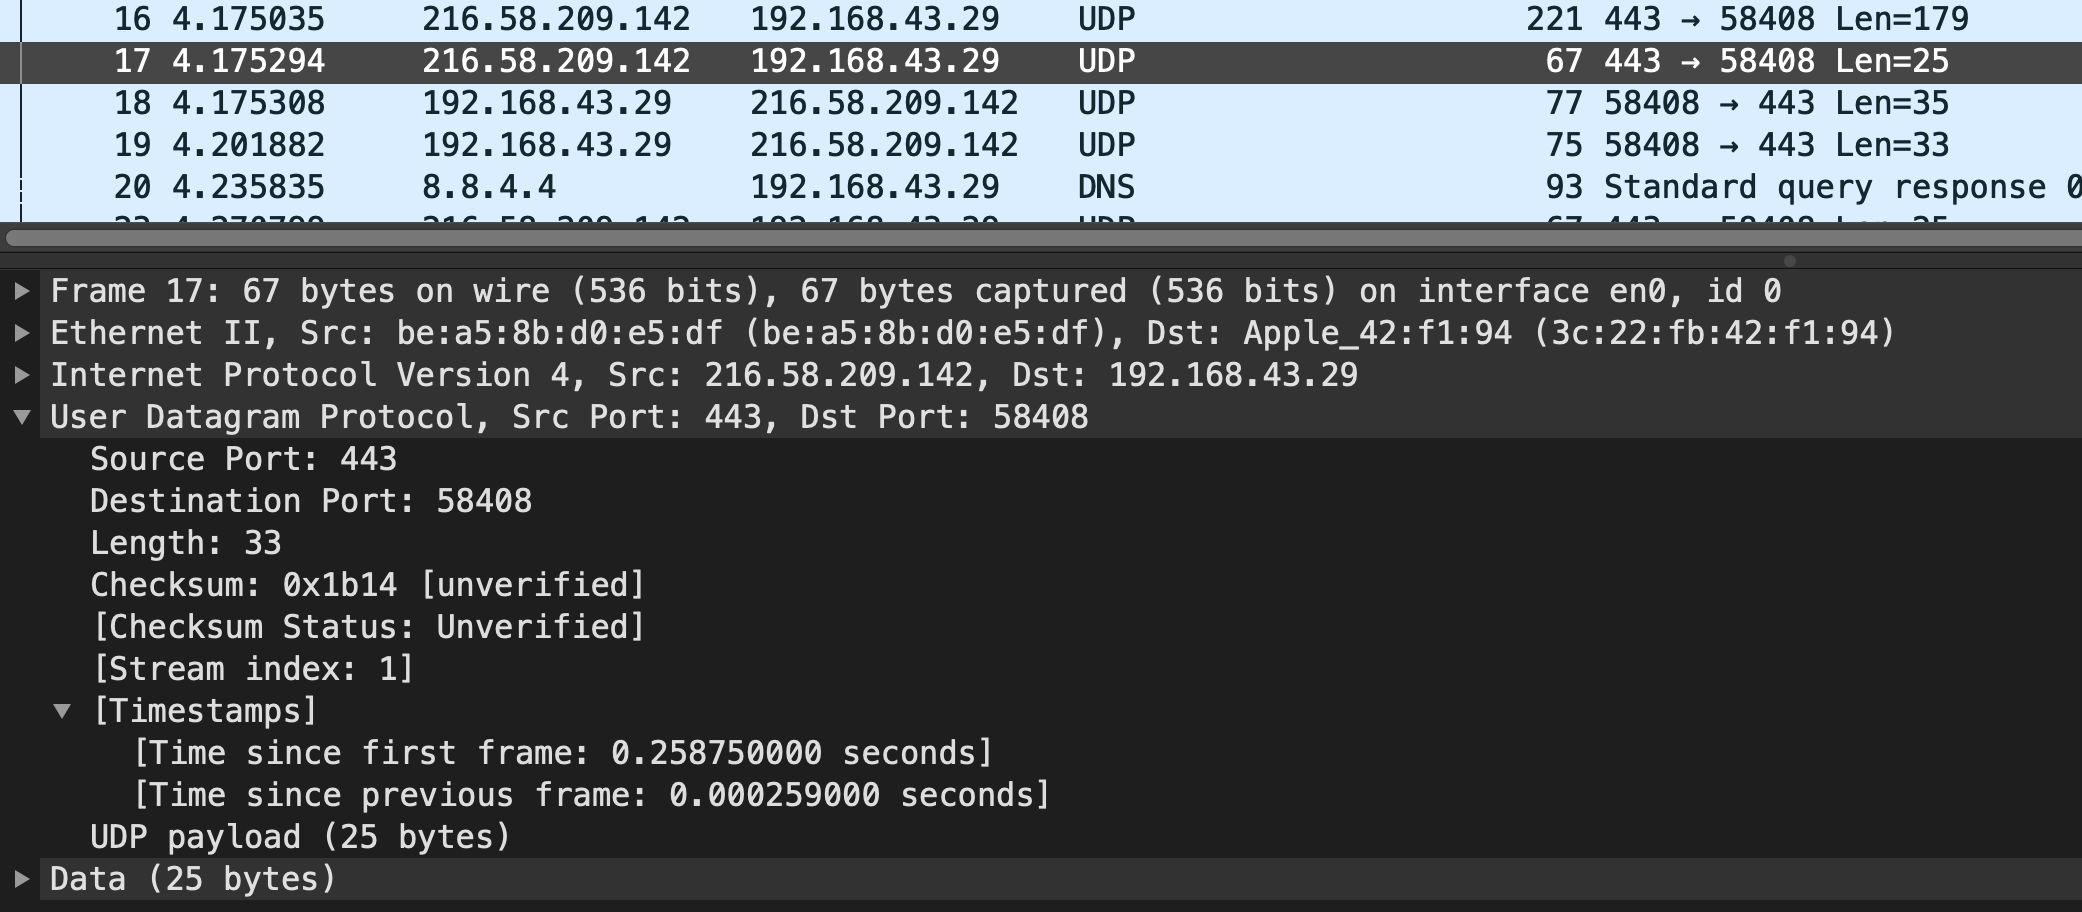
\includegraphics[scale=0.4]{u1}
	\lr{
	\paragraph{fields}
	source port, destination port, length, checksum
	}
}

2- \\\\

{
	\centering
	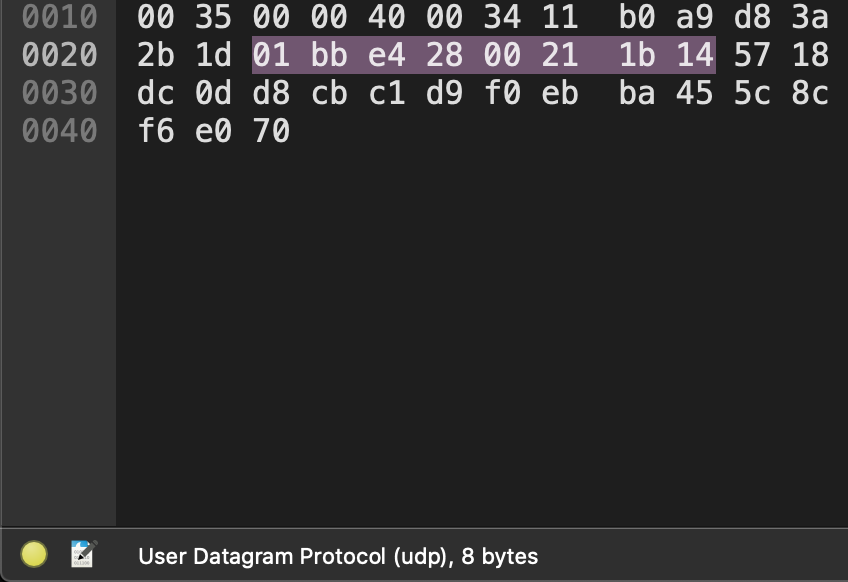
\includegraphics[scale=0.4]{u2}
	\lr{
	\paragraph{length of header fields}
	each 2 bytes in size, with a total of 8
	}
}

3- \\\\

{
	\centering
	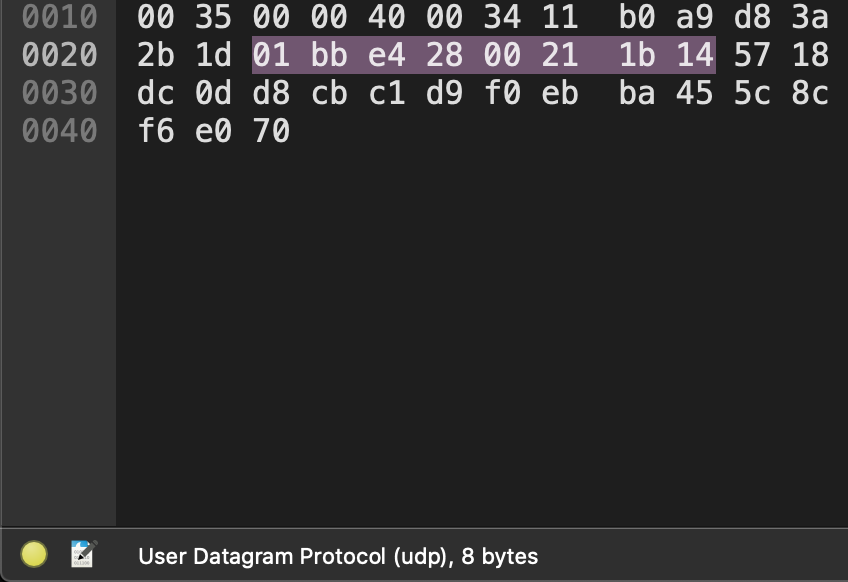
\includegraphics[scale=0.4]{u2}
	\lr{
	\paragraph{length field}
	it's sum of udp header length and payload (8 + 25 bytes payload)	.
	}
}
\\
\begin{latin}

\paragraph{4- max payload size} \\
\lr{
 2 bytes for showing length, resulting in $2^{16}$ distinct numbers.
(excluding 8 bytes for header)
}

\\\\
\paragraph{5- biggest port number}
$2^{16}$ bytes = 64 KB
\\
\paragraph{6- protocol number}
17 (0x11)

\paragraph{7- ports} ports from each ip stays the same. \\
{
	\centering
	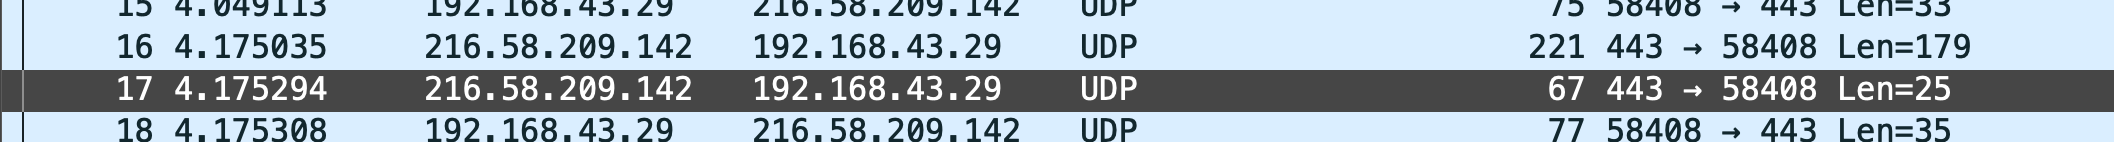
\includegraphics[scale=0.4]{u_l}
}

\end{latin}

\end{document}